\chapter{Coin cells}

From the impedance response of the battery and given an appropriate model, one an infer the internal workings of the system for control and prediction. Classical impedance spectroscopy is widely employed to estimate the state of charge (SoC) of individual cells or modules, and to indirectly extract information such as internal temperature or detect the occurrence of side reactions, such as lithium plating. More broadly, the internal resistance of the cell is strongly associated with its state of health (SoH). <- maybe this chould go in the introduction or method section and instead here go directly to the point of the experiment! The reader is already aware of the reasons.\\

In this chapter, I present the measurement of dynamic impedance of batteries during operation, continuously during the cycling lifetime. The aim is to demonstrate the advantages of impedance measurements under operating conditions compared to the classical stationary approach, in order to promote further research in this direction particularly in addressing the challenges of hardware implementation (for research or on-board control electronics) and the development of dedicated software solutions for the estimation and analysis. The acquired spectra are analyzed using standard methods, including distribution of relaxation times (DRT), transfer function parametrization, and statistical approaches.\\

For the experiments, I choose to work with a commercial reacharable Lithium-ion battery. The constrain was the total deliverable current of the electrochemical workstation at my disposition, equal to 500mA, that means 90mAh for each of the 6 channels if all are running simultaneously. Furthermore, for an immediate evaluation of the methodology the cycling life should not be too long (weeks is preferable than months). Assembling cells in-house was an option but it impacted reproducibility. The decision lent on the Panasonic ML2020 coin cell with the following characteristics:
\begin{itemize}
    \item Maximum theoretical capacity 45mAh;
    \item Positive electrode of Lithium Manganese oxide;
    \item negative electrode of alloy of lithium and aluminum;
    \item Electrolyte of ??? with no specified lithium salt.
\end{itemize}
The battery is meant for use as buffer for low power electronics and have a very limited self-discahrge. The manufacturer advices to recharge the battery with a current of 100uA and the suggested operational limits are between 1 and 3 V.\\

\section{Method}

The experiment here conducted was the measurement of dynamic impedance during a constant current - constant voltage (CCCV) testing profile, typical for testing of batteries performance and degradation in laboratory. To analyse the impact of the multisine perturbation on the cell, the same protocol was performed without any additioinal perturbation to the cycling drifts. To compare the impedance under operation and the stationary case, another set of measurments was performed in which the test protocol was interrupted, the cell rested and classic impedance acquired. All the experiments were conducted at room temperature.\\
The data were analyzed ??? Fitting of transfer function, DRT, long short-time memoery???

\subsection{Cycling test}
Voltage limit, current limits, c-rate, room temperature
For the classical testing of battery using the constant current -constant voltage technique, I used the voltage limits suggested by the manifacturer of 1-3V and a current of 4,5mAh, corersponding to a C-rate of C/10. After testing the capacity at C/20, 10 5 and 3 it was clear that the C/10 rate is the fastest that could possible extract all, or very close, the theoretical maximu charge of 45mAh. During the potentiostat step, the voltage is kept to a value of 3V with a lower current limit of 1mA,corresponding to C/45. I collected a dataset from 12 identical cells of the type ML2020 Panasonic syclend them with this protocol in a BioLogic battery cycler at room temperature. 
\subsection{Operando acquisition of stating impedance}
To obtain the impedance of the cella at different open circuit potential the same cycling protocol described in section above was here used with the addition of an interruption after 10\% of the total charge is flown in the cell (corresponding to 4.5mAh). When this charge limit is reached the system is hold at open circuit for 1 hour for relaxation an the classic impedance measured. The range is from 20kHz to 10mHz. 
\subsection{Real time acquisition of dynamic impedance}
For the measurement of the dynamic impedance, the electrochemical workstation was set to produce the same CCCV protocol as described above.\\
The multisine perturbation used here is from 10mHz to 100kHz, divided in two waveforms generate from two channels of the waveform generator. The waveform covering the lower band of the spectra is fro 10 mHz to 87 Hz created with a time step of  1e-3s(equivalent to 1000 Hz) and a period of 100s. The harmonics componing the frequency sequence are the one onbtained without intermuladulation, with 8 points per decade. The higher band of the spectra consisted of a range 
multisine from 100Hz to 100 kHz created with a time step of 1e-6 (1MHz) and a period of 10ms. In both cases the phases where indipendelty minimized via randomization repeated 200 times, keeping the lower value. \\
For the sampling of the voltage and current signals from the cell a picoscope of the series 4000 (two channels) was used. The acquisition frequency was 500Hz, twice the Nyquist frequency of the signals. For the online computation, a window of 100s was used, equal to the period of the multisine, the DFT performed to compute the impedance of the frequency band from 1Hz to 100kHz and the signals low pass filter with a simmetric Fermi-Dirac filter with bandidth 0.9 Hz and order 25 centered around 0Hz. The filtered signal was then resampled at 50Hz for storing. \\
The remaining part of the spectra from 10mHz to 0.8Hz was estimated offline using the Dynamic Multi-frequency Analysis with again a symmetric Fermi-Dirac filter centered at each frequency to analyze. The bandwidth is of 0.01Hz, the order of 8. Perform performing the analysis, both voltage and current signals were detrended using a simple linear baseline removal to reduce the effect of the drift.
\subsection{Analysis of impedance data}
Fitting of trasnfer function\\
- Correlation analysis of the coefficient\\
- long short-memory neural network \\
DRT\\
\section{Results}
From the regular cycling of the 12 identical coin cells I computed the total charge during discharging per cycle. The results, reported in figure...

\section{Discussion}

























\newpage
Identification of battery state

In this section it I described the work on the characterization of commercial coin cells though their life-time from their time-varying response. 
For this project I used a complete “battery”. In this introduction I would like to point out some terminology differences used in this chapter, \colorbox{BurntOrange}{following the discussion of paragraph??? between electrochemistry and battery science.}

\subsection{Choice of the cell}
With the intent of demonstrate the relationship between the time-varying impedance of a battery during standard operation and state of health, I decided to rely on commercial cells whit the assumption of a more consistent aging behavior compared to hand-made cells. Looking at the consumer market for Li-ion batteries one quickly relies that the capacity (or maximum charge) of this type of cells start from around 1Ah and goes up. The instrument at my disposal (BioLogic potentiost/galvanostat of the premium series) are capable of delivering a maximum of  500mA in total among the active channels. On the instrument with 6 channels that I intended to use for measuring the cells in parallel it means a maximum current per channel of 90mA. The only available rechargeable batteries that satisfies the maximum current limitation when cycled at 1C that I could find where the Panasonic ML2020 45 coin cell. Thier characteristics are reported in the table ???

These cells are base on MnO2 and  Li/Al alloy in a glycol based electrolyte. Manganese oxide is one of the first material used for the intercalation of lithium. It is cheap despite not the best in performance. Its drawbacks are : i) Lower energy density compared to more modern cathode materials; ii) Limited cycling stability, which can lead to capacity fade over time; iii) Lower operating voltage compared to other cathode materials, resulting in lower overall cell voltage; iv) Potential for manganese dissolution, especially at elevated temperatures, which can negatively impact battery performance.

On the megative electrode of such cells there is metallic lithium alloyed with aluminum. Lithium alloys quite well with aluminum (give some proof!!) giving less chances of dendride formation. The electrolyte is a not precisely specified salt in ??? solvent that possess a low conductivity, probably to reduce cell self-discharge, which is a characteristic underlined in their marketing  allowing for a maximum current of 4,5 mAh (equivalent to C/10) to extract the full 45mAh capacity of the cell. Such a limitation reveled to be significantly useful for this project. In fact the low current in the system produces a system close to linearity facilitating the separation of the component of the multisine perturbation from the main drift. Furthermore this cells posses a scarse cyclability at this c-rate (C/10) with a degradation of the capacity below 80\% of its original value in just 25 cycles, more or less; means circa 3 weeks of instrument time. Indeed these cells are meant as buffer for electronics components that use very little power. The raccomandare charging current from the manufacturer is C/200. For this project was a good platform to develop the software to control the instrumentation over a sufficiently long time-scale, testing and evaluating the stability of the algorithm while being able to spot di errors end implement the solutions in a matter of days.

\subsection{Performance test of the cell}

\colorbox{BurntOrange}{Put the test at lower  and higher c-rates}

\colorbox{BurntOrange}{The tests were performed in a battery cycler …..}

I was initially concerned by the possibility that the long term exposition of the cell to a multisine perturbation could accelerate aging. From a theoretical perspective the oscillation of the multisine is small enough to produce a negligible power and such a negligible heat generation at the interface of the electrode. To prove this point, 12 coin cells were tested through a constant-current-costant-voltage protocol with a current of 4,5mA, a voltage window between 1 and 3V and a a termination of the constant voltage phase when the current reaches 1mA. The discharge capacities of the cells is reported in Figure.

\begin{figure}
    \centering
    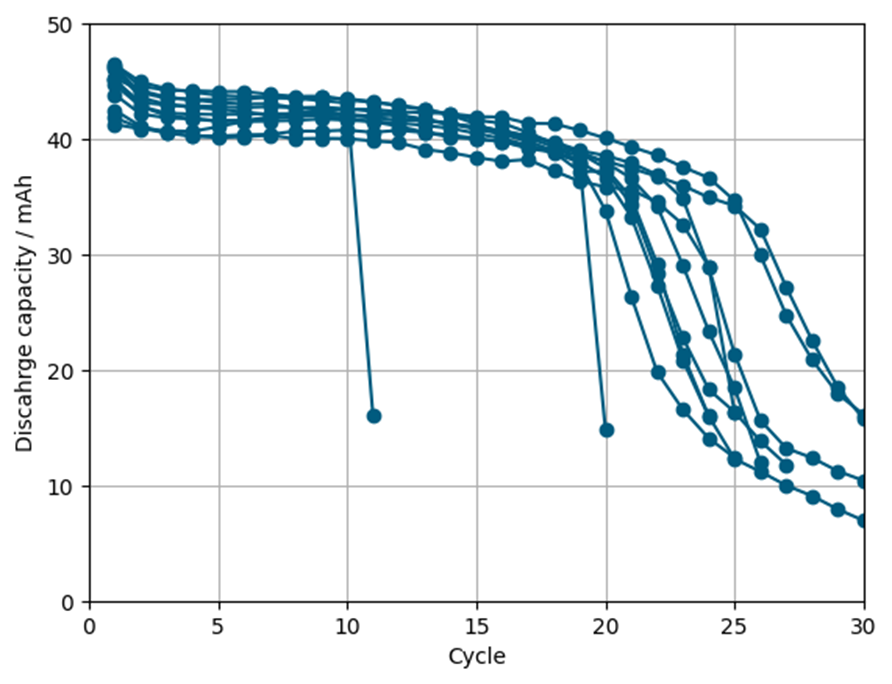
\includegraphics[width=0.8\linewidth]{figures/application4/image1.png}
\end{figure}

\subsection{Static impedance evaluation}

The static impedance for a new battery at the production voltage of 2.8V is reported in the figure.

\begin{figure}
    \centering
    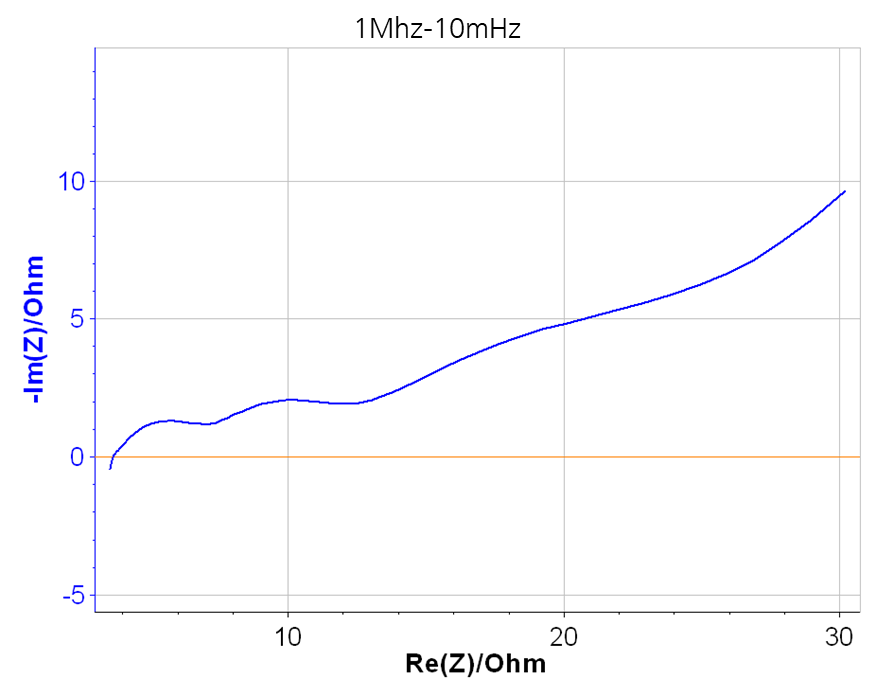
\includegraphics[width=0.8\linewidth]{figures/application4/image2.png}
\end{figure}

\colorbox{BurntOrange}{Plot the static impedance at different states of health and comment the time required to perform it.}

\subsection{Time-varying impedance acquisition}

Following, I performed a series of experiment using the multisine perturbation imposed during the constant-current-constant-voltage experiment maintaining the same experimental parameters. In this case the limits where chucked on the avarage value of the voltage or current over 30 seconds to compensate its oscillation; a control loop in the software was included for this task.

For this project, the experiment contemplate the combination of both a voltage and current controlled techniques therefore two multi-sine waveforms were prepared to be used during the two techniques. Both were composed of the same amount of sine waves of equal frequencies but the amplitude was designed differently to garante always an output signal with enough intensity for each frequency. The phases where choosen via iteration of random values to reach a low crest factor. The consideration for creating multi-sine are discussed in section ????. The lowest frequency in the multisine is of 10mHz while the highest of 1kHz. The waveforms where generated with a frequency of 5kHz and sampled with the digital acquisition device PicoScope 4000 or PicoScope 5000. The two series of devices have different amount of channels and more importantly different precision of the analog-to-digital converter (16 bits and 14 bits) although no effect on the quality of the extracted impedance was found. 

The two types of multi-sine, for the galvanostatic and potentiostatic experiment were both loaded on the memory of one channel of the arbitrary waveform generator. A control loop in the Python application is responsible of monitoring the running technique on the potentiostat and switch accordingly to the opportune multi-sine waveform on the generator.

The multi-frequency current and voltage signals where recorded and streamed to the memory of the Python application which saves them in separate folders per techniques. The time-varying impedance was then estimated independently from the multi-frequency signals of each technique using the Dynamic Multi-Frequency Analysis following the removal of the baseline in the non-constant (on the median) signal. The filter used for the analysis was a Symmetrical Fermi-Dirac Function with a bandwidth of 0,01Hz and n-value of 8. 

The discharge capacities for the cells under continuous multi-sine perturbation are reported with the previous set in Figure XX; it can be concluded that no significant acceleration of the degradation is related to the use of multi-sine.

\begin{figure}
    \centering
    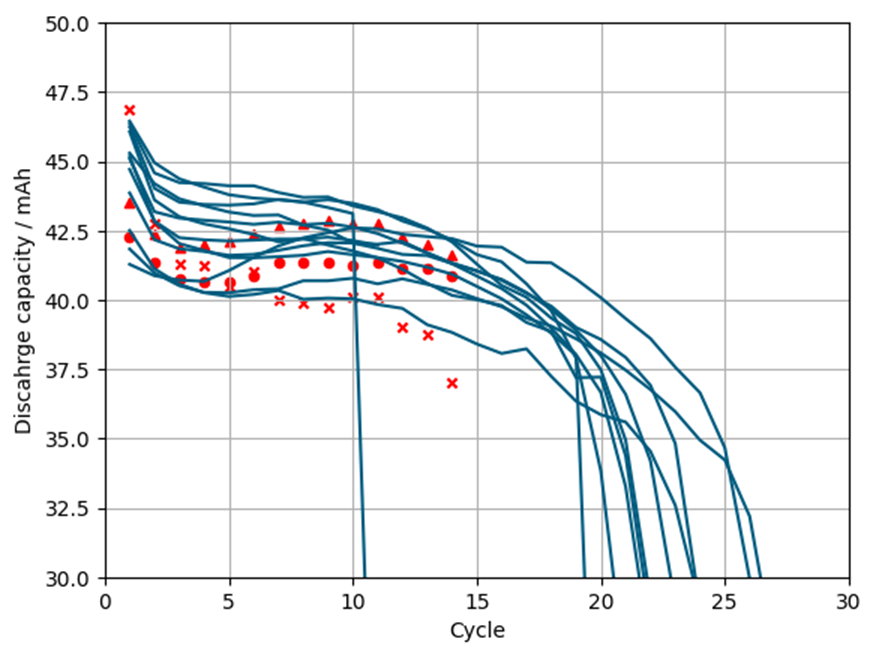
\includegraphics[width=0.8\linewidth]{figures/application4/image3.png}
\end{figure}

Now a qualitative evaluation of the time-varying impedance estimated form the Dynamic Multi-Frequency Analysis will be given. First, I analyzed the shape of the first discharge curve and the impedance at same depth of discharge. The comparison is reported in figure.

\begin{figure}
    \centering
    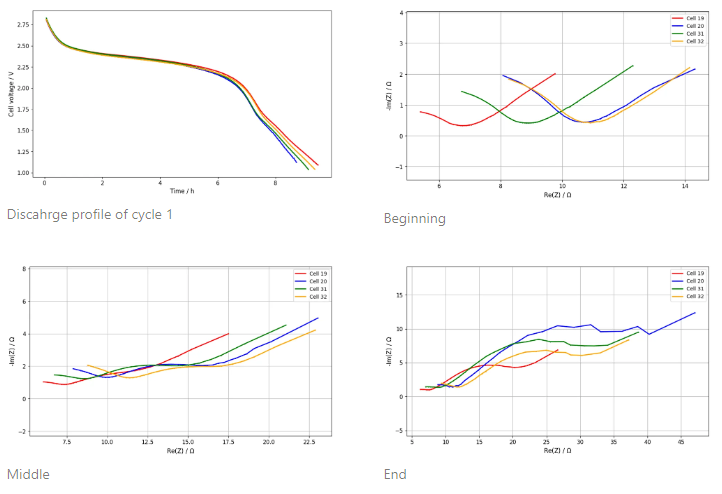
\includegraphics[width=\linewidth]{figures/application4/image4.PNG}
\end{figure}

The cells exhibit similar capacity and equal voltage profile for the first half of the discharge. The last part of the discharge varies a little bit in its over-potential, probably due to the increased and uncontrolled roughness of the surface of the negative electrode during alloying. Considering the potential of alluminium and lithium alloying at 100mV vs Li/Li+ thermodynamically, with such high overvoltage I expect the potential of the negative electrode to go easily below zero and cause a parallel lithium deposition reaction. I believe this is also the cause of such fast lost of capacity, for the low cycling efficiency for the dissolution of lithium deposit smaller than critical radius, and events of short circuit. Figure ???  also shows the impedance of the cells at different depths of charges, circa at the beginning, in the middle and at the end of the discharge. Here a first observation come, the impedance of the cells at the beginning are different of around 20-30\% while the voltage profile looks identical. This is a first advantage of the impedence of showing characteristics that are invisible at the low frequency scale (means direct current) but might have a significant impact on the performances. It is interesting to notice the blue and yellow lines to be very similar from the beginning to the end, while the red curve showing always a smaller impedance value. It is not surprising to se the highest discharge capacity (visible as longer time to discharge) for the cell with the lowest impedance (red line).

The shape and magnituse of the impedance for the four cells reveal a different response for the consequent cycles. In the Figure XXX it are reported

\begin{figure}
    \centering
    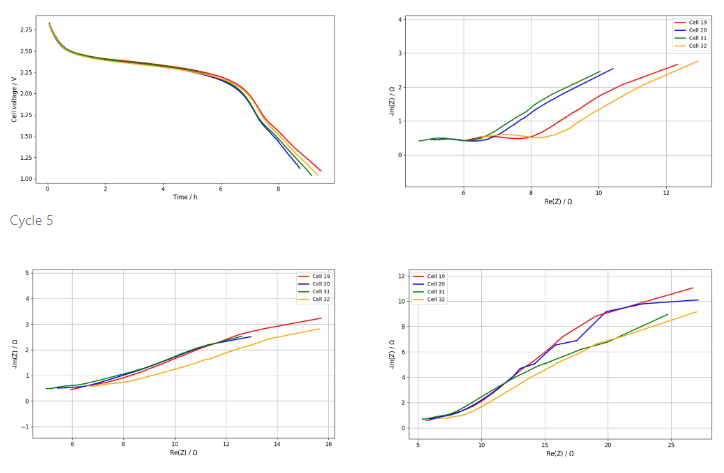
\includegraphics[width=\linewidth]{figures/application4/image5.PNG}
\end{figure}

The time-varying impedance of the cells conserve a similar a similar trend until the aging start to accelerate faster. Here we also assist to a larger discrepancy between the cells in terms of both discharge capacity and impedance. See Figure XX.

\begin{figure}
    \centering
    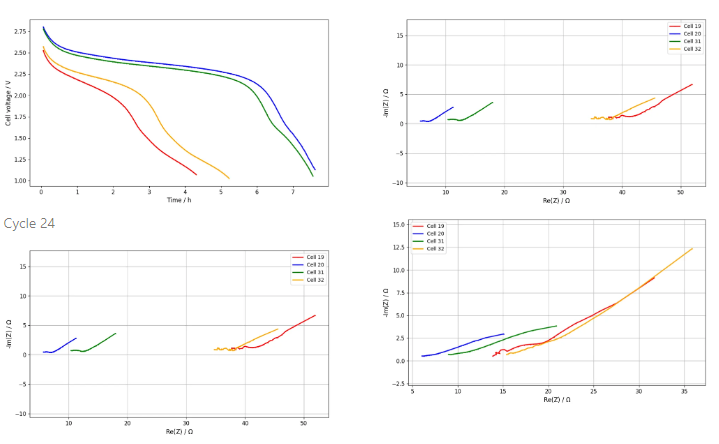
\includegraphics[width=\linewidth]{figures/application4/image6.PNG}
\end{figure}

The time-varying impedance of a system is a particularly big dataset that can be seen as two dimentional, as a function of time, or three dimensional as a function of charge and cycles. The latter is in my opinion the most informative being the cycling of a battery similar to a seasonal time series. The voltage and impedance of a cell as a function of the charge represent the state of charge while their dependency with the cycle number represent the state of health. Both informations are much informative to acquire and it is exactly the scope of this project. Nontheless such a rich information (considering also that the impedance is complex) is impossible to fully display on paper as 2D immages. In this section, some snapshots of the full movie, to ripropose the picture-movie analogy from the introducion, are provided to the reader after a filtering of the author. This is a intrinsic problem of data visualization that belong to any science. ????

During the data analysis process, interactive figures where fundamental to find interesting variation on the system impedance, but still in a qualitative way, just base on the eyeballing. A way to codify the information in a lower dimensional is needed to demonstrate the relationship between impedance and the states of the batteries, both of charge and of health. This is the topic of next section.

\subsection{regression of rational polynomial}

colorbox{BurntOrange}{Despite begin so challenging to measure the impedance of a system, especially in non-stationary condition, it is only half of the job. To make all the work worth, one must extract information about the system under study.}

A transfer function, as is the impedance, is in its analytical form a rational polynomial as shown in the introduction. After estimating the impedance spectrum of a system over a set of frequencies from an experiment, it comes natural to want to deduct the transfer function that output such results to be used as model of the system and simulate it behavior under different operating conditions than the experiment. For this work we combined some ideas from statistics and system theory to find in a robust approach to find such function among the many possible. The first idea is to have a generalized model of additive terms, i.e. polynomial, as from the Generalized Additive Models but non linear and especially both rational and of incremental power. This translates in a model of such a form:
\begin{equation}
    f(x) = \frac{a_0+a_1x+a_2x^2+...+a_kx^k}{b_0+a_1x+b_2x^2+...+b_kx^k}
\end{equation}

This is identical to the definition of transfer function. It is convenient to fix b0 to 1 to have always a finite value. The second idea come from Information theory and it is about the choice of an opportune k which means to have a criteria to decide when to stop adding term to the polynomial. In fact, a fitting gets always “better”, or the residues of the regression are smaller, with the increase of the number of parameters. On the other hand the new parameters have no physical significance or do not univocal define the system. In this case we talk about overparametrization. The problem of estimating the original information from a signal with uncertainty is at the core of a branch of statistics and Computer science called Information Theory. The amount of information, translated in common means as degree of freedom of a system, is converted to a quantity called Entropy of information. Minimizing this quantity brings to the correct number degrees of freedom for a model to describe the data. This concept was formalized by Akaike and further developed in the years. 

When searching for the correct transfer function model for the case of time-varying systems it is also expected that the coefficients (a and b) of the rational function continuously change during the evolution of the system physiacal chacartesitics without any sudden jump or going to zero. This scenario can very when the model is overparametrized in certain parts of the dataset (for example at the beginning or at the end of the experiment). In fact the parameters space of the fitting procedure becaome rougher with many close minima. The solution might not anymore be unique. Thi is clear when fitting the single impedance spectra from a time-varying experiment one after the other. To ensure smoothness and continouity of the fitting parameters, a penalty factor can be added to the object function of the minimization.  For this work we used a penalty on the second derivative of the parameters and this means adding one non-free paraemeter on the function. The choice of this parameter has of course a great influence on shape of the costa function hyper-surface and so the minimization procedure. A value too big don’t allow the parameters to vary until exactly fitting them while a value too small make the penalty negligible. The objective function to minimize in now the sum of the residues for the fit of all the spectra in the dataset analysed (i.e. the time-varying impedance of one discharge) plus the penalty factor. The problem defined this way has a very high dimensionality and could not be solved with standard solver for its uge memory consuption. For this projecy I use once again the library pymultipleis that take advantage of JAX virtual mapping to split the problem in smaller problems and efficiently parallelize it on the machinne. Furthermore the autodifferentiation capabilities reduce the compution time. \colorbox{BurntOrange}{The working principles of the library are described extensivelly in the introduction.}
\colorbox{Green}{The fitting of the model where conducted } on the admittance using the modulus as weighting factor. This helps the convergence to the absolute minimum giving less importance to the lower frequency that carry higher uncertainty.
To decide over the correct model and penalty factor value for an opportune model, I compared the different information criterium values of multiple optimization run in which I screened the rational function of increasing order k and eight smoothing factors for each, one value per decade from 1e-6 to 1e4. I repeated the regression for each of the four cells and the results are summarized in figure XX.


\begin{figure}[h]
\newgeometry{outer=10mm}
    \centering
    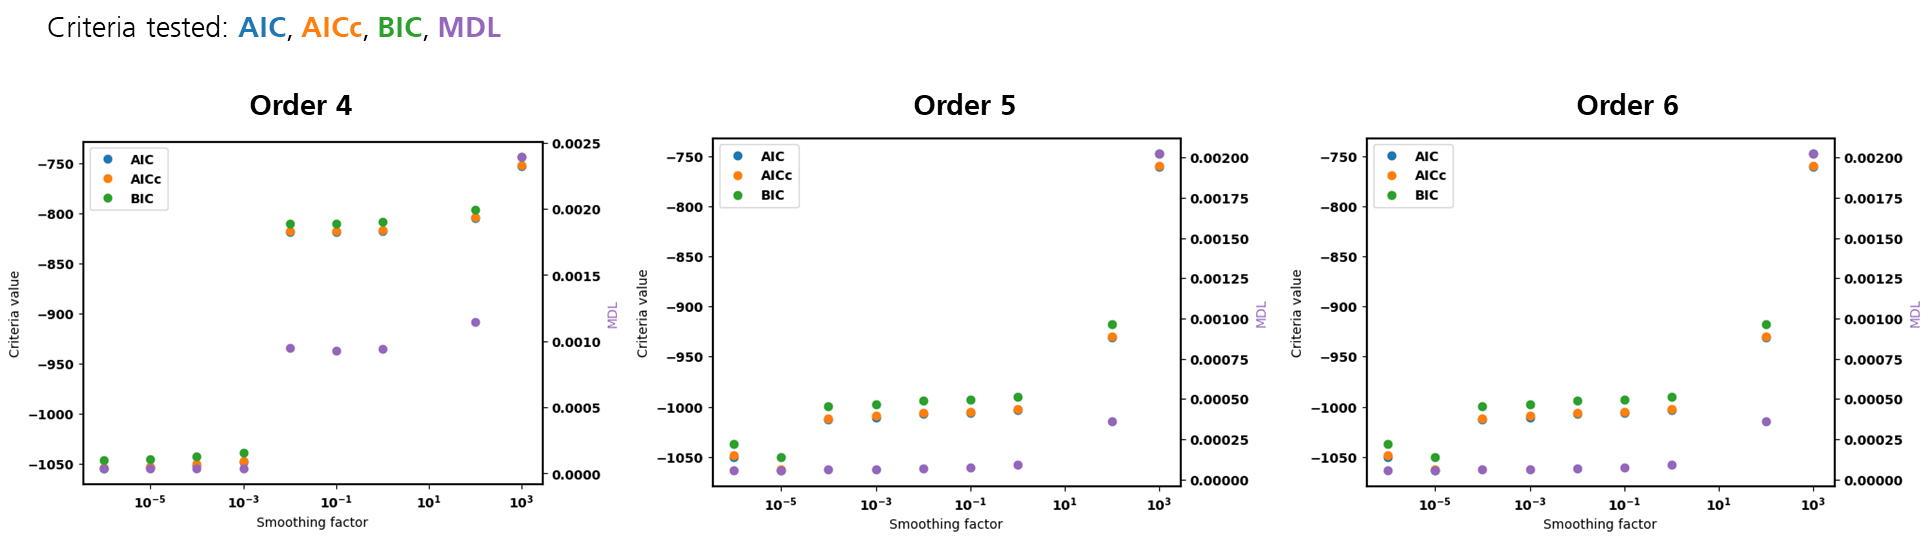
\includegraphics[width=\linewidth]{figures/application4/image7.png}
\restoregeometry
\end{figure}


\begin{figure}[h]
\newgeometry{outer=10mm}
    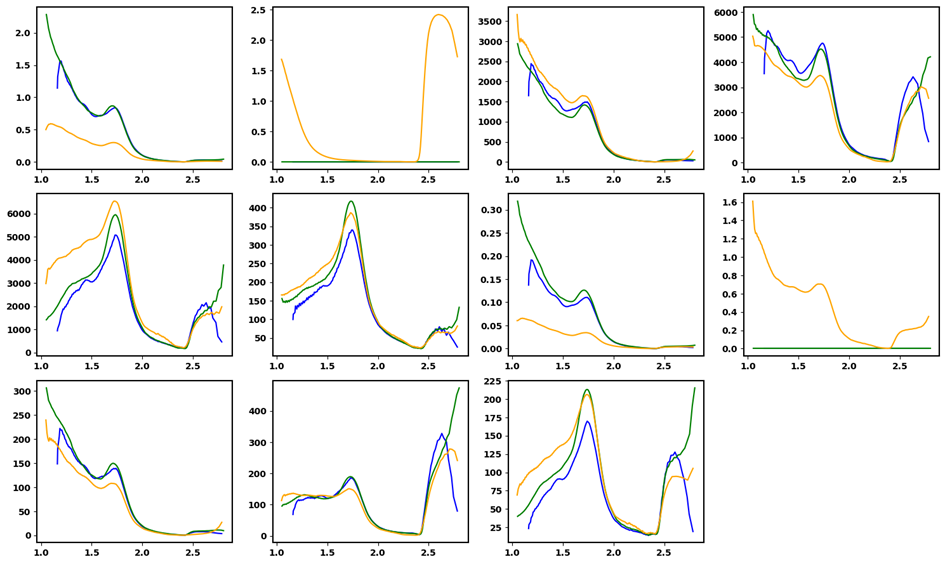
\includegraphics[width=\textwidth]{figures/application4/image8.png}
\restoregeometry
\end{figure}

From the previous figure it is clear that some of the parameters follow the exact same trend. Those are in fact correlated and should not me considered in the count of the degrees of freedom.

\begin{figure}[h]
    \centering
    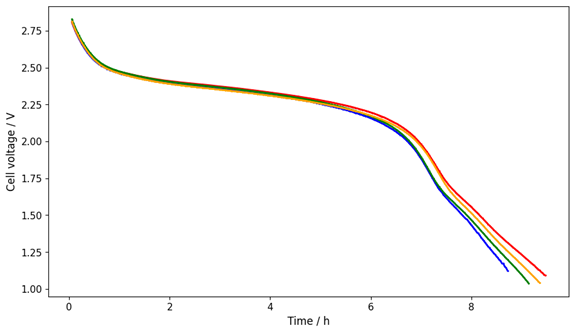
\includegraphics[width=\linewidth]{figures/application4/image9.png}
\end{figure}

The figure shows how the coefficients of the rational polynomial for k=5 evolves during the first discharge of the cell. Each of them have 2 or 3 distinct peaks centered at 2.6V, 1.7V and 1.3V. This values correspond to the change in steepness of the voltage profile. colorbox{BurntOrange}{This is more clear analysis the differential voltage curve.}

Once identified the proper model, the time-varying impedace for the life time of the battery was fitted producing the result in figure XX. From the picture it is clear the evolution of the parameter with the state of helath and state of charge. This parameterazation though ration polynomial regression allowed to visualize the time-varying impedance from one cell at one glance. The complex-valued impedance is transformed in real valued parameters.

\begin{figure}[h]
    \centering
    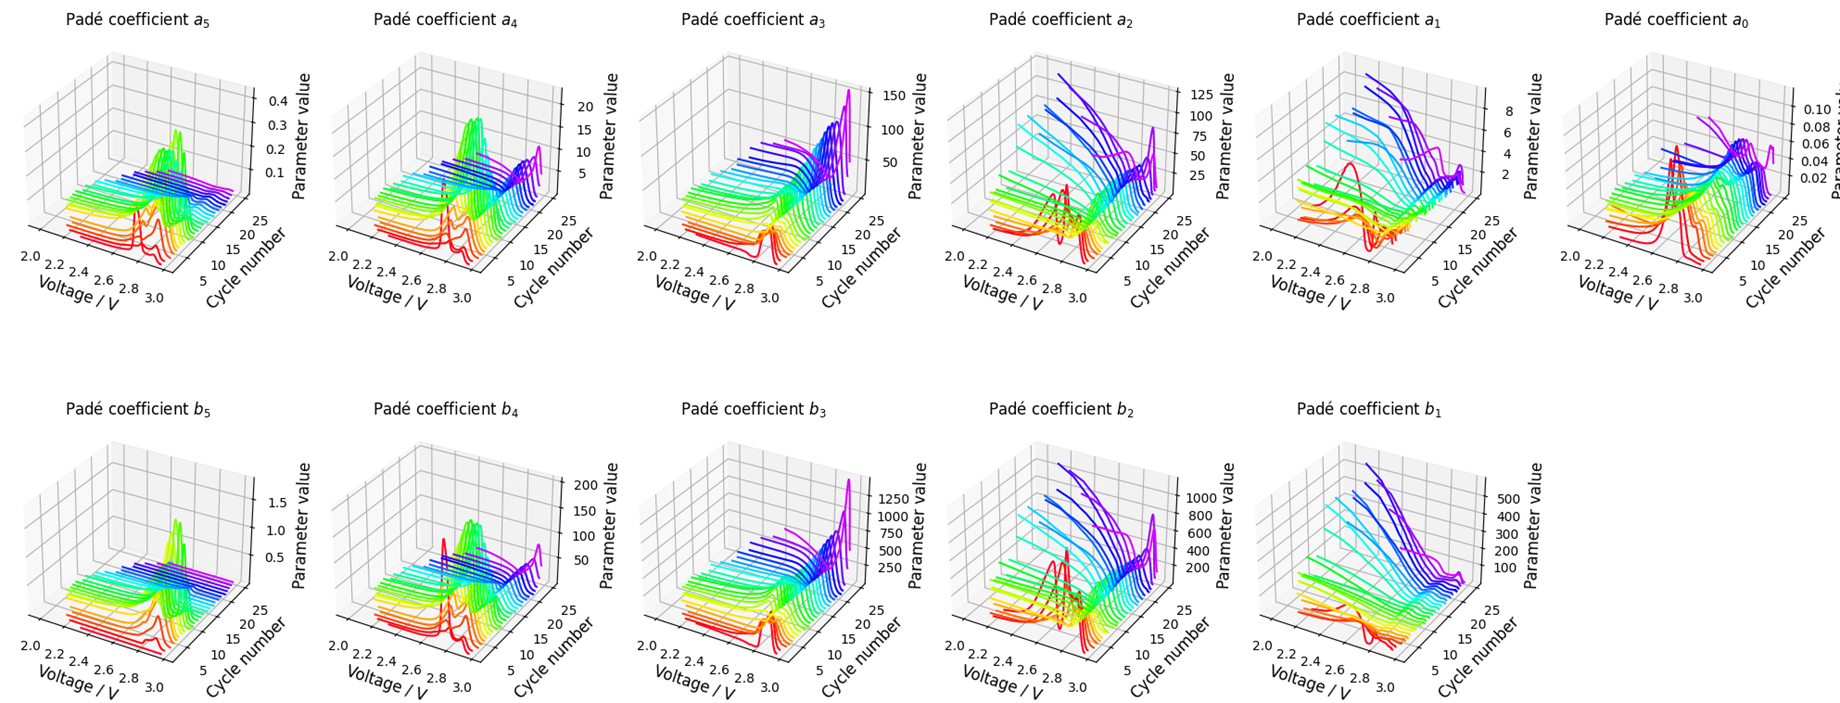
\includegraphics[width=\linewidth]{figures/application4/image10.png}
\end{figure}

\subsection{Associating measurement values with battery state}

The goal of this project is to demonstrate a relation between the impedance and battery state, ideally to use the data at one point of the cycling for the forecasting the rest. One of the most important information any user needs to have is the end of life of the device. It is not only practical for the user but represent a great economical value for the second life expectancy of a battery module. 

\newpage
\chapter{Identify lithium plating on graphite}
With the experience gained working on the projects described in the previous two sections, I was curious on the possibility of identify lithium plating in situ during reduction of the graphite though time-varying impedance. This is a huge topic, especially in the last years where company achieved (es. StoreDot) extreme fast charging. Fast charging, while enabiling a greater diffusion of electric veichles for the convience of it, should be use sparcelly. \colorbox{BurntOrange}{As described in the introduction}, chargin with high urrent densities pushes the potential of the negative electrode much lower than its themodynaic values to a point where lithium reduction is possible. Fast charging a battery every cycle inevitably reduced the life of the device. It is interesting though to know what happens after one fast charge cycle to the graphite electrode and if the impedance can retrive some information. The set-up used is similar to the one used for the project regarding silicon carbonitride and the mechanisms of sodium intercalation; I assemble a three electrode half cell in pouch format with natural graphite electrode and microscopic electrodeposited electrode, discharge the cell at 1C without any potential limitation but rather time limitation (i.e. charge) and then performed consecutive non-stationary impedance experiment in galvanostatic mode with increasing current density.

\subsection{Cell assembling}
For this project the working electrode was a graphite slurry of SBR and water doctor bladed on copper foil. The counter electrode was a square of lithium foil 22x22x?? mm (99.?? \%, Sigma Aldritch). An insulate copper wire current collector with diameter of 130um was produces with the same method described in the section before and the cell assemble using two glasfiber separator with the refernce copper wire between them, placed in such a way to have the exposed copper area in the center of the electrode area. 300 uL of electrolytic solution LiPF6 in EC:DMC 1M with 2\% of VC was poured in the cell and the device underwent 2 cycle of under-pressurization of 10 mbar to remove gasses from the pores while allowing the permeation of the liquid. The cell was sealed wit a coffe bag under a pressure of 10 mbar. \colorbox{Blue}{Transform in pascal}

\subsection{Time-varying impedance measurements}

\begin{figure}[h]
    \centering
    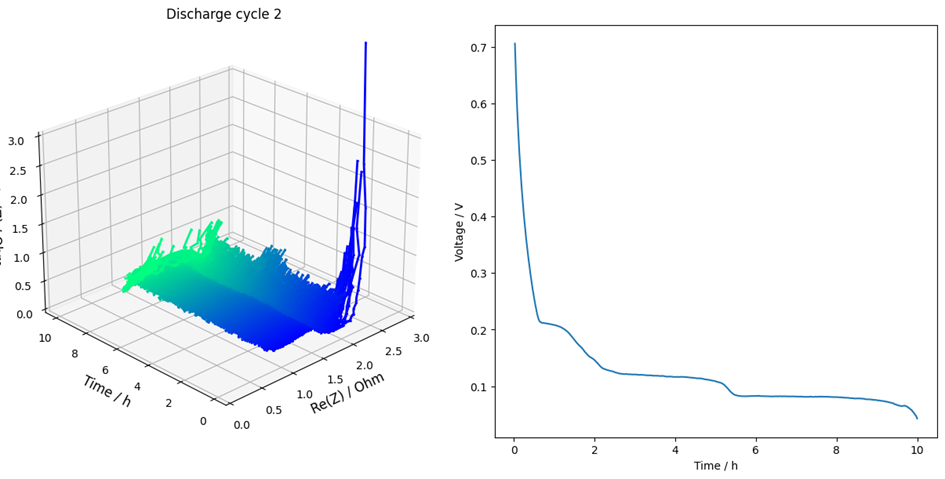
\includegraphics[width=\linewidth]{figures/application5/image1.png}
\end{figure}

\begin{figure}[h]
    \centering
    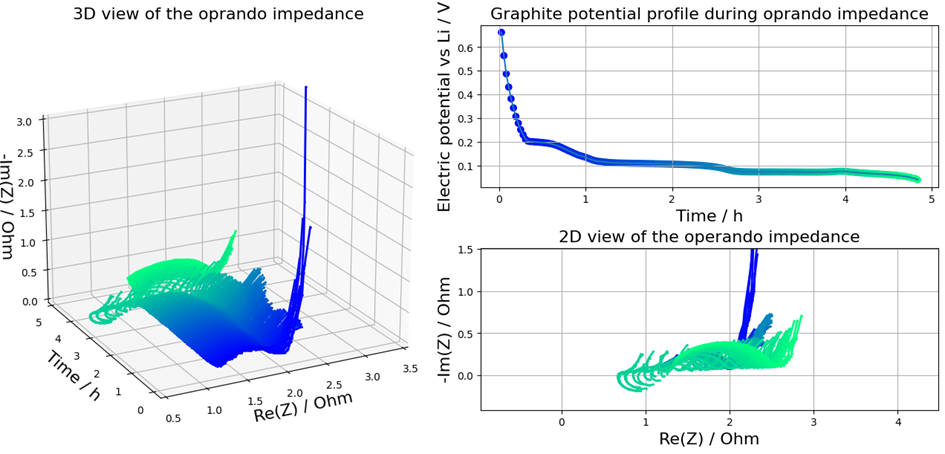
\includegraphics[width=\linewidth]{figures/application5/image2.png}
\end{figure}

\begin{figure}[h]
    \centering
    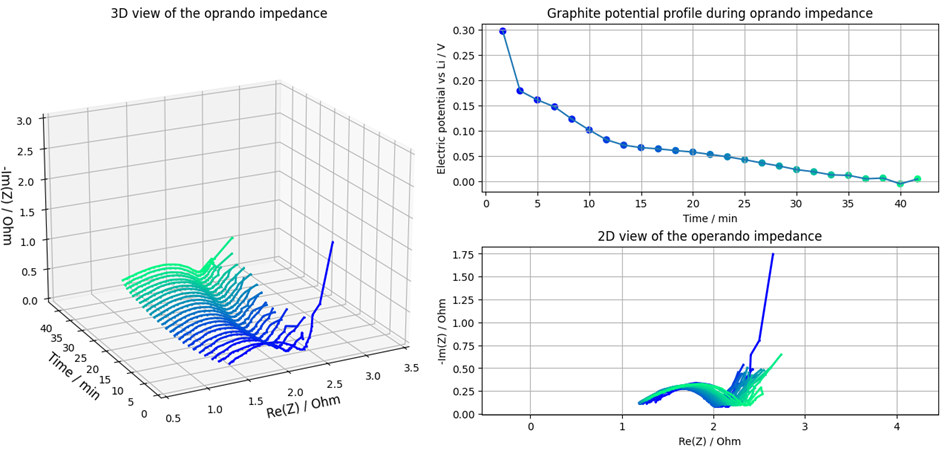
\includegraphics[width=\linewidth]{figures/application5/image3.png}
\end{figure}

\begin{figure}[h]
    \centering
    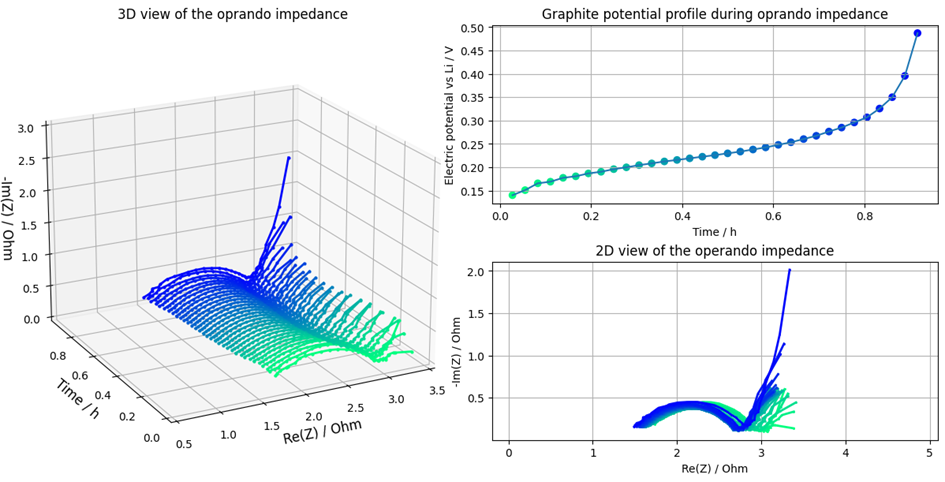
\includegraphics[width=\linewidth]{figures/application5/image4.png}
\end{figure}

\begin{figure}[h]
    \centering
    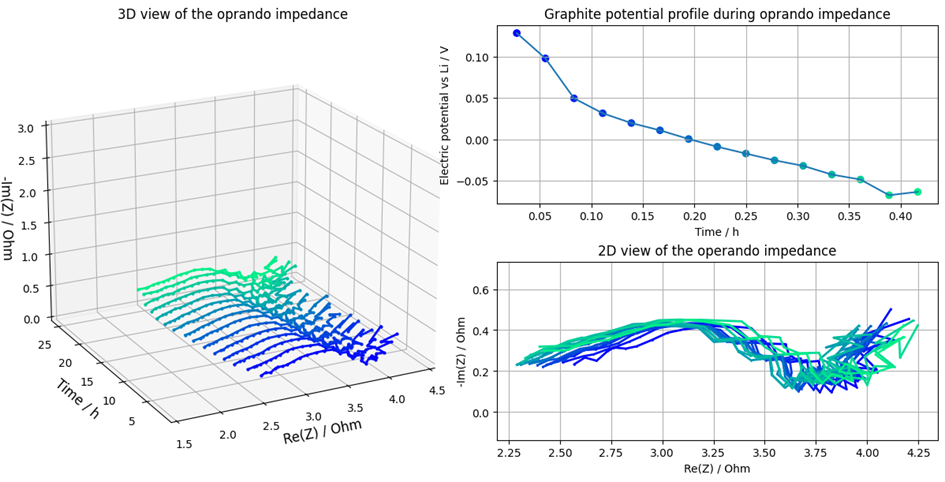
\includegraphics[width=\linewidth]{figures/application5/image5.png}
\end{figure}

\begin{figure}[h]
    \centering
    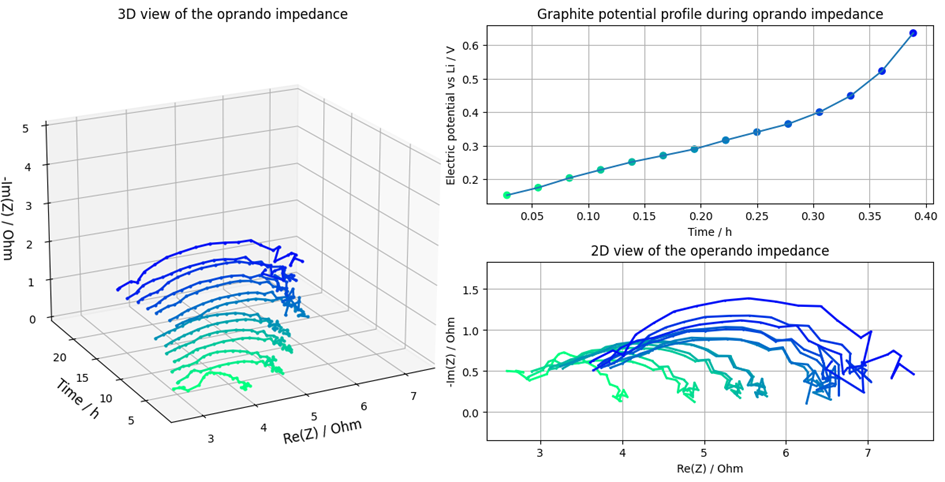
\includegraphics[width=\linewidth]{figures/application5/image6.png}
\end{figure}

\begin{figure}[h]
    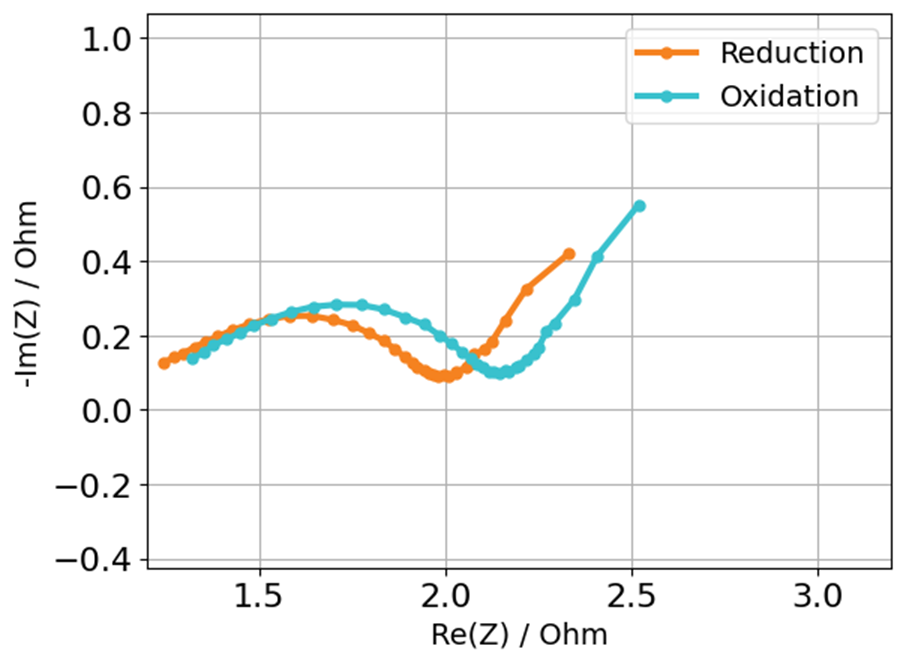
\includegraphics[width = 5cm]{figures/application5/image7.png}
    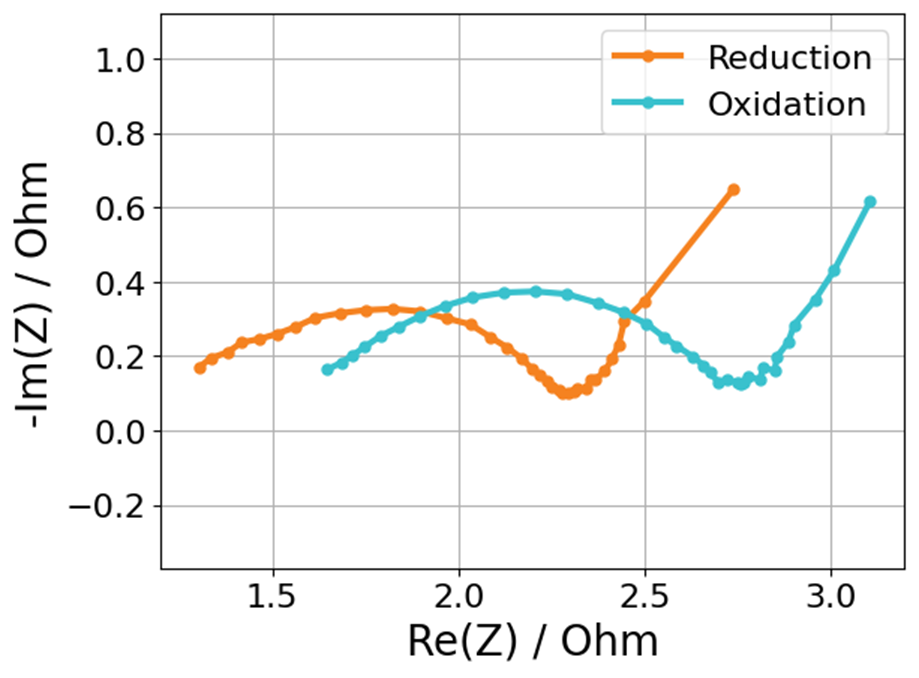
\includegraphics[width = 5cm]{figures/application5/image8.png}
\end{figure}

\begin{figure}[h]
    \centering
    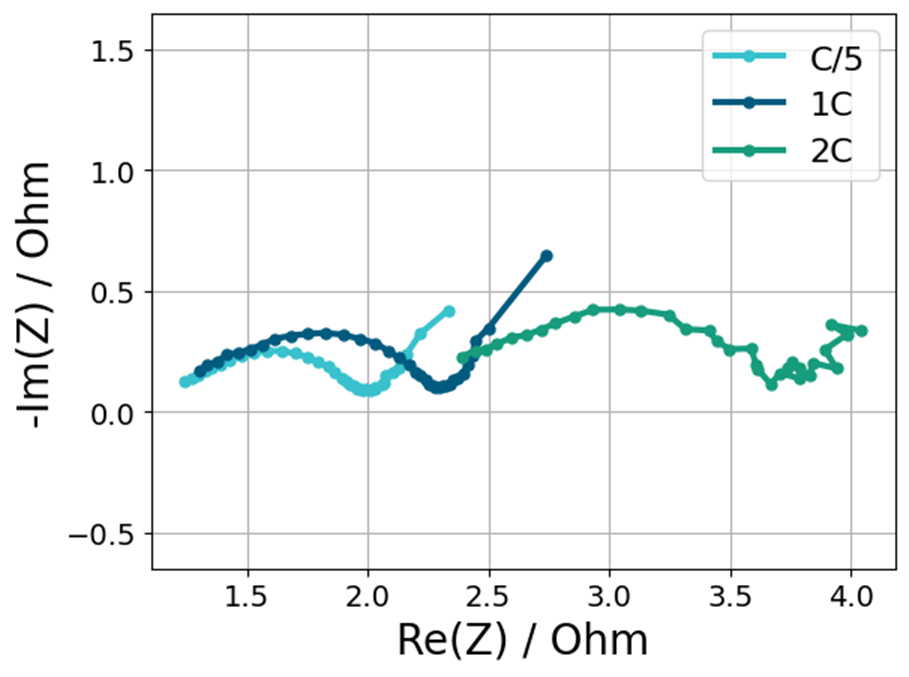
\includegraphics[width=0.7\linewidth]{figures/application5/image9.png}
\end{figure}